%%
%%  Department of Electrical, Electronic and Computer Engineering
%%  MEng Dissertation - Addendum B: Supplementary analyses (B.1 embedding space, B.2 crowd size and AP@OKS)
%%
\chapter{Supplementary Analyses}
\label{appendix_supplementary}

\section{Embedding-space visualisation}
\label{appendix_embedding}

\begin{figure}[H]
    \centering
    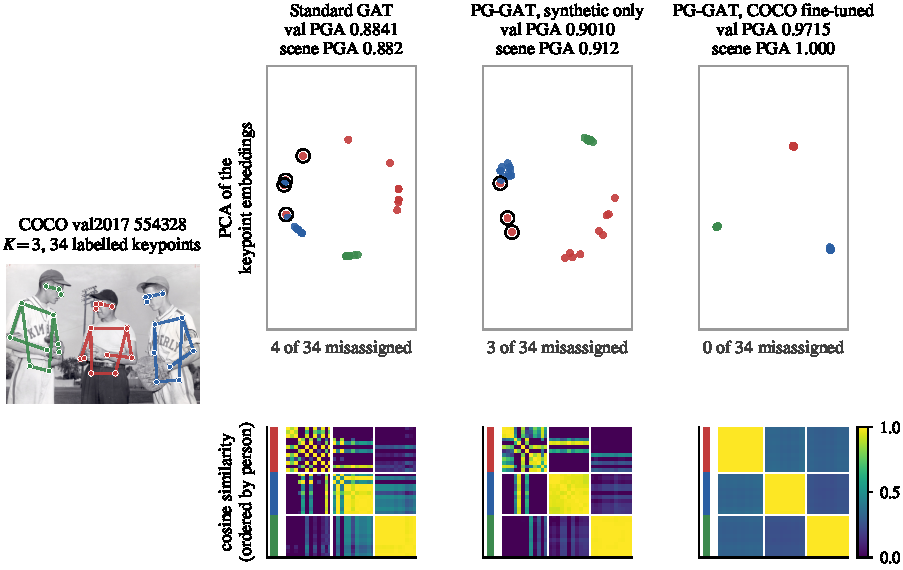
\includegraphics[width=\linewidth]{figures/embedding_space_pca.pdf}
    \caption[Per-keypoint embeddings for one COCO scene under three checkpoints.]{Per-keypoint embeddings of COCO \texttt{val2017} image 554328 ($K=3$, $34$ labelled keypoints)
    under the standard GAT baseline (run \texttt{jkd1ln4a}),
    the synthetic-only PG-GAT (\texttt{08d0ffde}),
    and the COCO fine-tuned headline PG-GAT (\texttt{b5noyg7t}).
    The top row shows the first two principal components of the embeddings, coloured by ground-truth person;
    keypoints assigned to the wrong person by the $k$-means read-out are ringed.
    The corresponding per-scene PGA values are $0.882$, $0.912$, and $1.000$.
    The bottom row shows the cosine-similarity matrices of the same embeddings,
    with keypoints ordered by ground-truth person.}
    \label{fig:embedding_space}
\end{figure}

Figure~\ref{fig:embedding_space} shows the per-keypoint embedding of one COCO scene at three stages of the
investigation:
the standard GAT baseline of Section~\ref{sec_res_baseline},
the synthetic-only PG-GAT selected by the architecture sweep of Section~\ref{sec_res_pggat_sweep},
and the COCO fine-tuned headline checkpoint of Section~\ref{sec_res_coco_ft}.
The scene is selected by a fixed rule rather than chosen for visual effect.
Among the \texttt{val2017} scenes containing three to five people and at least ten labelled keypoints per person,
it has the three per-scene PGA values closest to the corresponding dataset-level COCO validation results
($0.8841$, $0.9010$, and $0.9715$).
A two-dimensional principal-component projection is used because it is linear and reproducible.
Non-linear projections such as t-SNE separate the clusters even for the baseline embedding and vary between runs,
making them less useful for this comparison.
The cosine-similarity matrices show the relationships in the original embedding space without projection.
For this scene,
mean within-person cosine similarity increases from $0.582$ to $0.761$ and then $0.999$ across the three checkpoints,
while mean cross-person similarity is $-0.062$, $-0.075$, and $0.298$, respectively.
The fine-tuned model therefore maps the keypoints of each person to an almost identical direction while keeping
different people below the contrastive margin of $\gamma=0.5$,
rather than forcing different-person embeddings towards opposite points on the unit hypersphere.

\section{Grouping accuracy and AP@OKS against crowd size}
\label{appendix_crowd}

\begin{figure}[H]
    \centering
    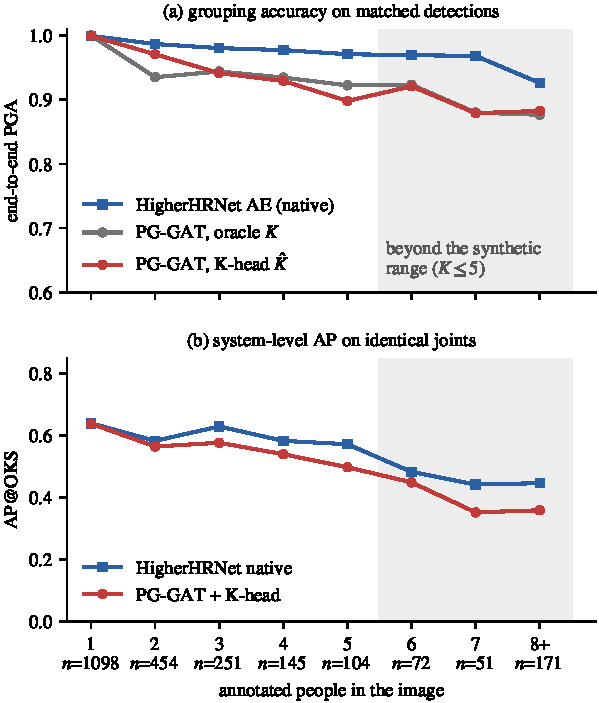
\includegraphics[width=0.7\linewidth]{figures/crowd_size.pdf}
    \caption[End-to-end PGA and AP@OKS against annotated person count.]{End-to-end PGA and AP@OKS against the number of annotated people in each image using HigherHRNet detections.
    (a) PGA on the matched detections of the $2{,}165$ scored scenes from Section~\ref{sec_res_e2e},
    comparing HigherHRNet's native associative-embedding grouping, PG-GAT using the annotated $K$,
    and PG-GAT using the K-head prediction $\hat{K}$.
    (b) AP@OKS over all $5{,}000$ COCO \texttt{val2017} images for the native grouping and autonomous PG-GAT pipeline
    using the same pooled joints, evaluated separately within each person-count bin using the COCO evaluator.
    The final bin contains images with eight or more annotated people,
    the shaded region marks counts beyond the $K \leq 5$ range used during synthetic training,
    and $n$ gives the number of images in each AP bin.}
    \label{fig:crowd_size}
\end{figure}

Figure~\ref{fig:crowd_size} breaks the end-to-end results down by annotated person count and supplements the PGA
analysis with AP@OKS.
Panel~(a) reports the PGA from Section~\ref{sec_res_e2e} for each person count.
Panel~(b) evaluates HigherHRNet's native grouping and the autonomous PG-GAT pipeline using AP@OKS under a protocol that
differs from the PGA evaluation in three ways.
First, all $5{,}000$ COCO \texttt{val2017} images are evaluated rather than only scenes containing matched detections.
Second, every pooled detection above the $0.1$ confidence threshold enters the PG-GAT graph,
including detections that do not match an annotated keypoint.
Third,
pose instances are assembled from the resulting $k$-means clusters by retaining the highest-confidence detection for
each joint type, with surplus same-type detections discarded.
The predicted person count is constrained by the number of available detections,
$K=\max(1,\min(\hat{K},N))$,
and both methods use the same instance-score convention.
Under this protocol, native grouping reaches $0.540$ AP on the pooled joints,
compared with $0.492$ for the autonomous PG-GAT pipeline, a difference of $0.048$ on identical input joints.

Two measured effects help explain this difference.
First, the errors are concentrated in more crowded scenes, which contribute multiple person instances to AP.
For the $2{,}052$ images containing one to five annotated people, the AP difference is $0.029$;
for the $294$ images containing six or more, it increases to $0.076$.
Across the individual bins,
the difference grows from $0.001$ for single-person images to $0.088$ for images containing eight or more people.
The latter counts also lie outside the $K \leq 5$ range used during synthetic training.
This concentration is less visible in the per-image mean PGA but can be seen directly in panel~(a).

Second, the $0.1$ pooling threshold removes low-confidence joints that HigherHRNet's native refinement stage retains.
These joints contribute $0.043$ AP to the native result:
using the detector's full output raises its AP from $0.540$ on the pooled joints to $0.583$ under the single-scale,
no-flip evaluation used here,
compared with the published $0.671$ result with flip testing.
Simply lowering the pooling threshold to zero does not recover the difference for PG-GAT.
Doing so increases the K-head's mean prediction to $4.07$, compared with $3.44$ instances produced by the detector,
and reduces AP to $0.467$.
Using the detector's own instance count instead raises this result to $0.497$,
leaving a $0.086$ difference from the detector's full native output.

Several properties of the AP protocol are consistent with the remaining difference,
although they are not isolated experimentally.
Unmatched detections enter the graph and can displace matched joints during instance assembly;
an incorrect person count can affect an entire predicted instance rather than only individual keypoint assignments;
and a cluster containing joints from two people can produce both a low-OKS prediction and a missing person.
At the $0.1$ protocol threshold, however, person-count estimation is not the main source of the observed AP difference.
Replacing the K-head prediction with the annotated count gives $0.483$ AP,
while using the detector's own instance count gives $0.484$, both below the K-head result of $0.492$.

Panel~(a) also refines the person-count result discussed in Section~\ref{sec_disc_modularity_autonomy_autonomy}.
The K-head's overall advantage over the annotated count is concentrated in two-person scenes,
where PGA is $0.971$ compared with $0.935$ using annotated $K$.
At four and five people the relationship reverses:
the K-head reaches $0.929$ and $0.898$, compared with $0.934$ and $0.922$ using annotated $K$.
PGA therefore remains the primary metric for the grouping experiments for the reason given in
Section~\ref{sec_res_e2e_ap}:
it isolates assignment quality on matched keypoints,
whereas AP@OKS also incorporates detection recall, localisation error, person-count errors,
and the rules used to assemble keypoints into pose instances.